\section{Electrical}

The ASV is powered by two 12.8V 8Ah LiFePO4 batteries connected in parallel. A 100W solar panel mounted above the electronics enclosure charges the batteries directly, with a blocking diode to prevent reverse current during low-light conditions.

Power is distributed through three buck converters that step the 12.8V battery voltage down to 5V. One converter powers the Raspberry Pi, another supplies the SpeedyBee F405 V4 flight controller and GPS, and the third is dedicated to the servo motor. All components are placed inside a waterproof enclosure without mounting hardware.

\begin{figure}[H]
    \centering
    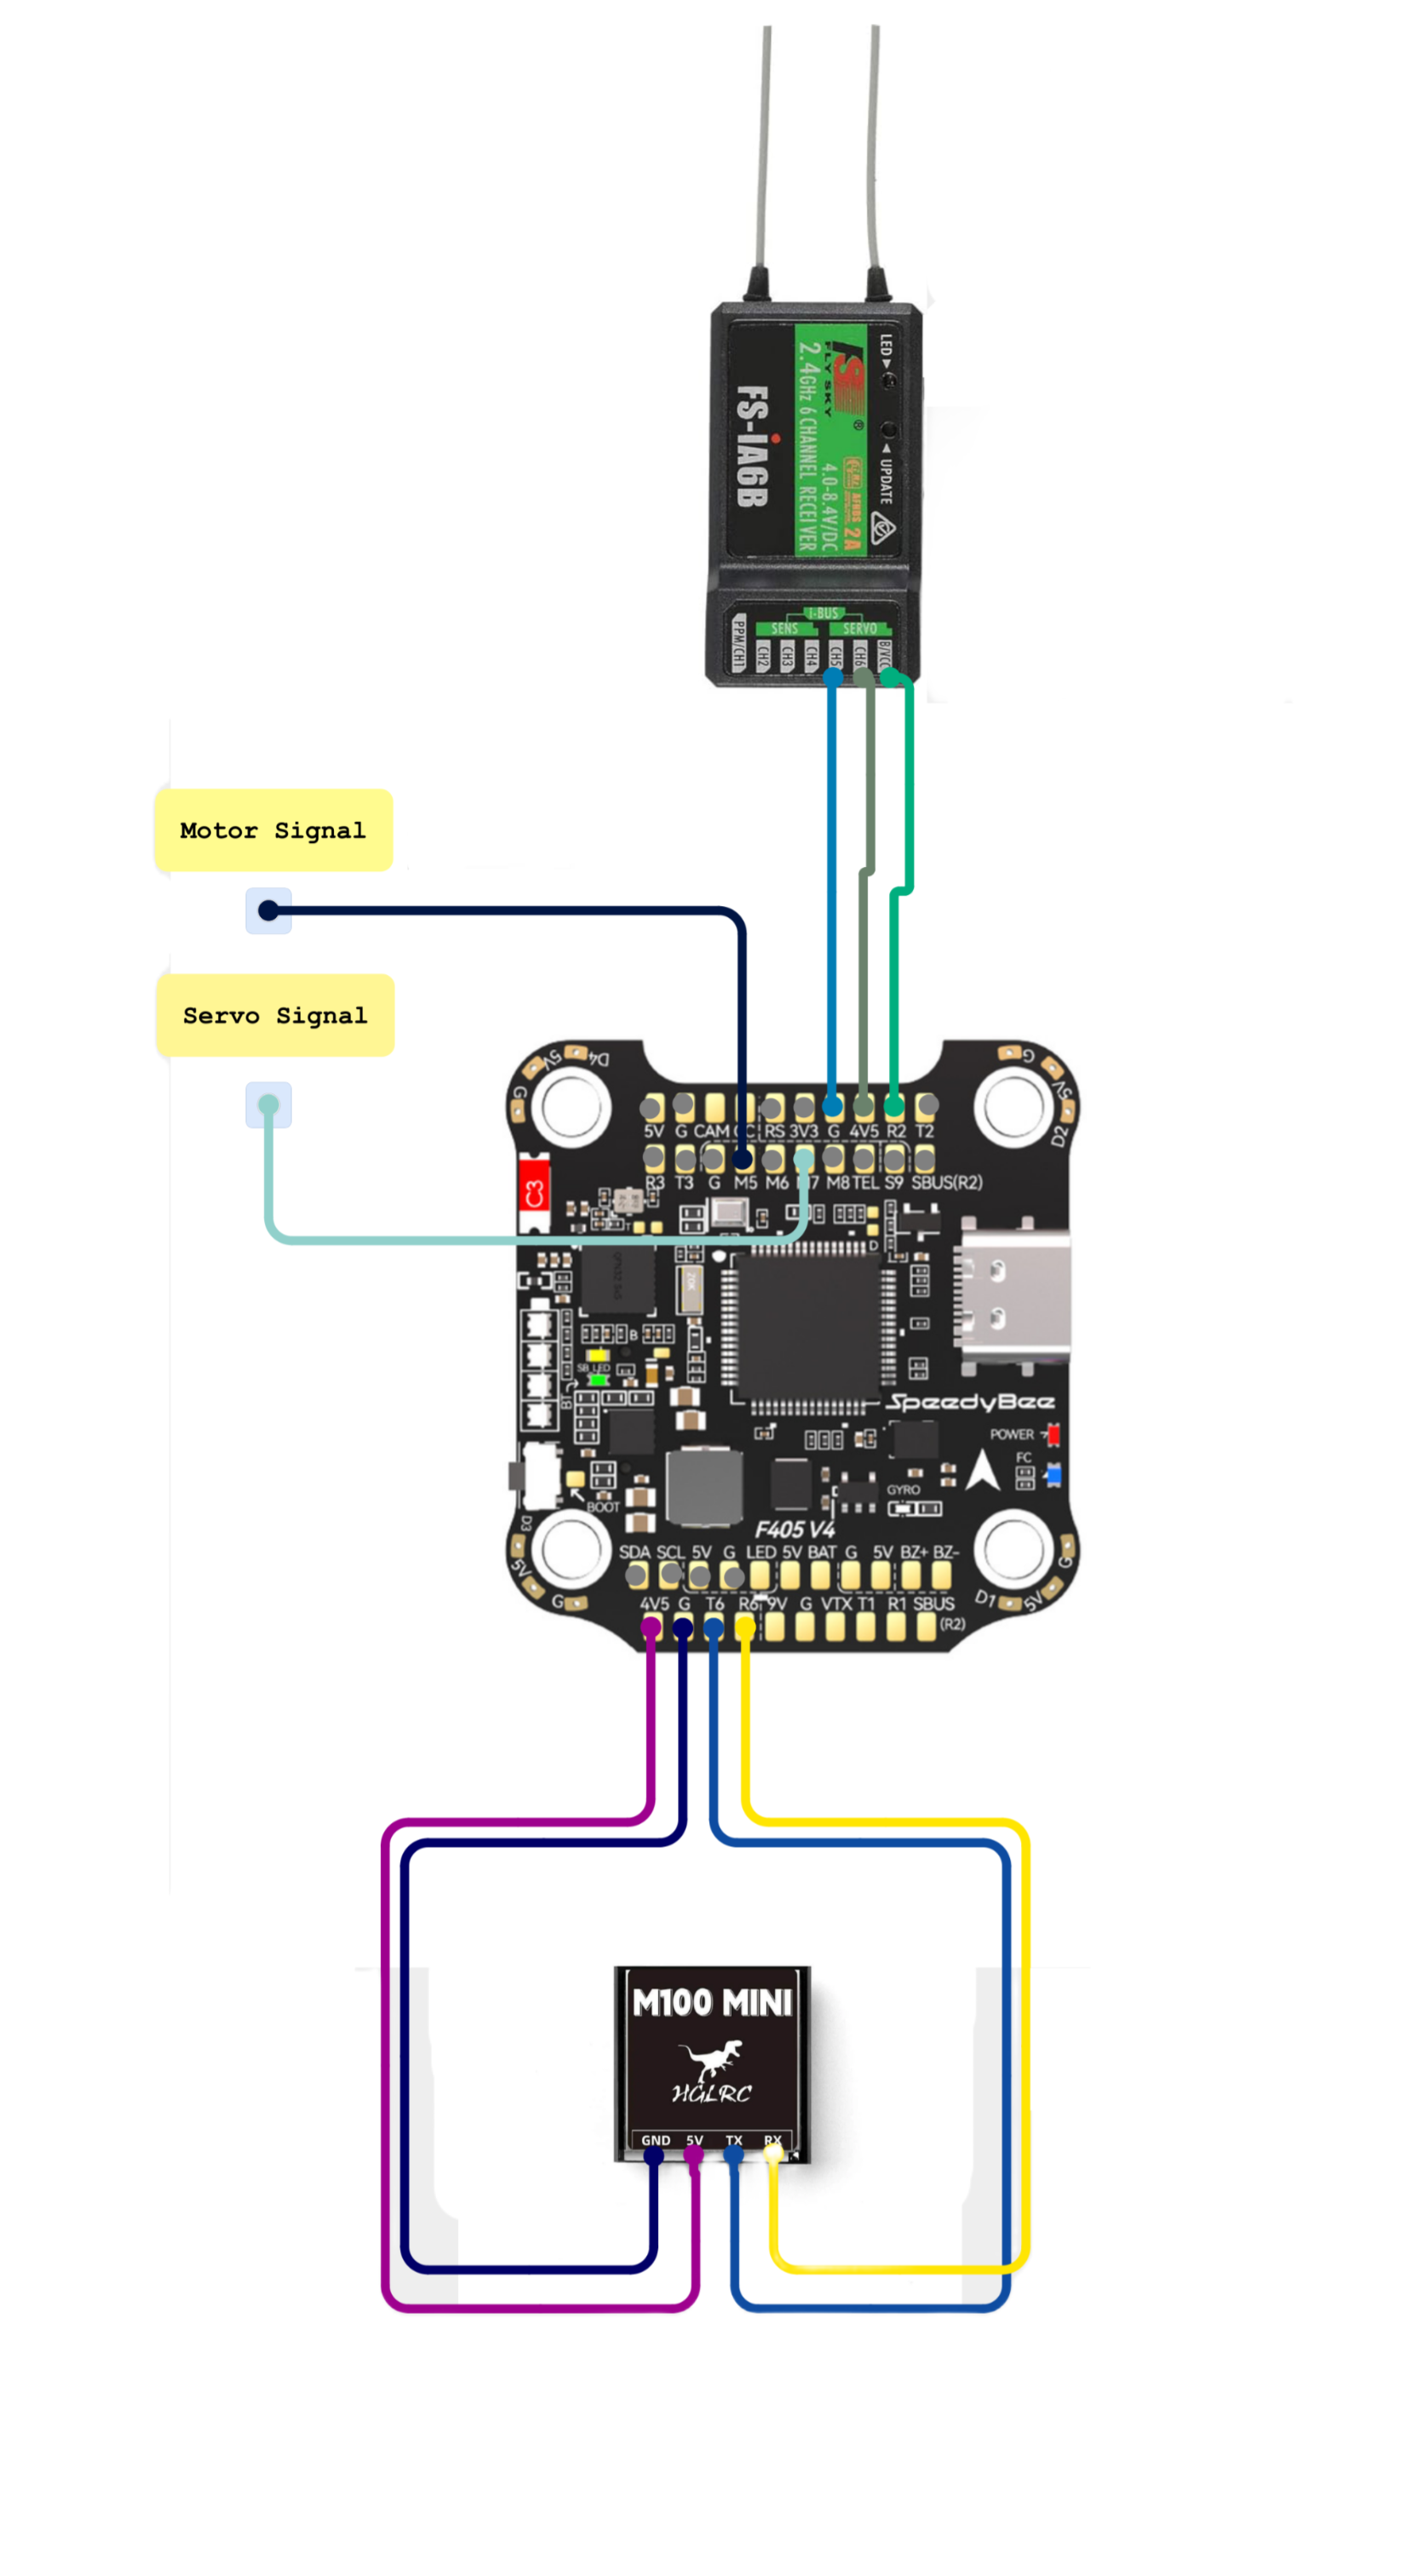
\includegraphics[height=10cm]{speedybee.png}
    \caption{Schematic of the SpeedyBee F405 V4 flight controller and its connections.}
    \label{fig:Speedybee}
\end{figure}

The SpeedyBee F405 V4 flight controller runs iNav firmware and handles both GPS waypoint navigation and motor control. It outputs PWM signals to the brushed DC motor and rudder servo and receives location data from a GPS module. The GPS is soldered directly to UART6 on the flight controller: TX from the GPS is connected to RX6, and RX from the GPS is connected to TX6. A FlySky FS-iA6B receiver is soldered directly to the RX2 pad on the flight controller for SBUS communication, enabling manual RC override when needed.

To generate a magnetic field, a 40 Hz sine wave is created by a prebuilt signal generator and passed through a power amplifier. The amplified signal drives a large copper coil wrapped around the boat's structure, producing a low-frequency magnetic field detectable by submerged sensors.

All electrical connections are made using soldered wires. Power and signal lines are routed manually inside the enclosure. Signal and high-current paths are physically separated to minimize noise. Fuses are installed on the battery output lines to protect critical components from short circuits.

The electrical system is simple, modular, and designed for ease of repair and future upgrades. Components can be swapped or rewired without requiring full system disassembly.